%EXP

\subsection{Experimental Setup}

The 218 publicly-available and labeled patients were downloaded from NCBI and converted to FASTQ format using the SRA toolkit, and labeled according to the labels on EBI, as described in the Materials section. Each read was assembled with SOAPdenovo2, with the k-mer length set to 51, reads cut off after 100 base pairs (original length of 180 base pairs), and the average insert size set to 350 in accordance with the reported average insert size reported in the MGWAS study \cite{qin041012}. Assembly for each file took 7-30 minutes, depending on the file size, and each patient was assembled in parallel. Combining the files into one file took 12 minutes, and clustering with UCLUST took 10 hours and 51 minutes. Without assembly first reducing the size of the data, clustering would not have been feasible. SVM-light took 10 minutes and 17 seconds to run.

\subsection{Results For Bag/Patient Labels}

Temp

\subsection{Deriving Instance "Labels"}

\begin{figure}[t]
\centering
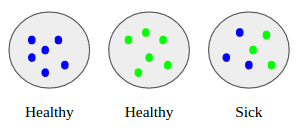
\includegraphics[scale=0.5]{./instance-labels.png}
\caption{This diagram illustrates why static instance labels are not sufficient for phenotype prediction. A patient with 6 of the blue microbe or 6 of the green microbe may be healthy, while a patient with 3 of each is sick. Static instance labels cannot capture this relationship. This is also explored by Amores in his MIL taxonomy \cite{amores13}.} \label{instance-labels}
\end{figure}

One of the benefits of using Multiple Instance Learning methods is that we can attempt to discover instance "labels". In fact, we did not attempt to apply static, unchanging labels to individual reads or clusters, since organisms are affected by their interactions with each other. For instance, a patient with X amount of microbe A or X amount of microbe B, but not with X/2 amount of microbe A and X/2 amount of microbe B. This is illustrated in Figure \ref{instance-labels}. This example is very simplified, but it explains why static instance labels are insufficient.

However, we can infer from the SVM decision boundary which clusters appear to be most relevant to the disease diagnosis. Since feature vectors are multiplied by the weight vector of the decision boundary to determine the label of the patient, we can assume that clusters with the highest weights in the weight vector are most relevant to the disease diagnosis. For instance, if the Ith scalar in the weight vector is has the highest value of any of the weights, then cluster I is likely to play a major role in the disease. Similarly, the most negative weights in the weight vector indicate clusters whose presence in a patient indicates that they likely do not have the disease. Because the data is metagenomic, the clusters represent both phylogenetic and functional similarity, so identifying the most relevant clusters can help discover more about the pathology of the disease. For Type 2 Diabetes, which is a complex phenotype and a disease that is both common and deadly, this is potentially quite valuable.